\chapter{Introduction}\label{chap:Intro}

Graphs are widely used to represent complex information such as social networks, chemical compounds, World Wide Web, logistic networks, bioinformatics, etc.
% They are used due to their unique ability to efficiently represent complicated relational information.
% \SV{Club the two sentences?}
Graph algorithms have applications in diverse areas like molecular engineering, social sciences, operations research, computer science, and many more.
Formally, a graph $G$ is defined as a collection of vertices $V$ and edges $E \subseteq V \times V$ represented as $G=(V,E)$, where vertices represent entities and an edge represents relation between a pair of entities that are its endpoints.

Subgraph Enumeration is a fundamental problem in graph theory that aims at finding all instances of a given query graph $G_q$ in a larger data graph $G_d$.
Formally, given a query graph $G_q$ and data graph $G_d$, the objective is to find all instances of subgraphs of $G_d$ that are \textit{isomorphic} to $G_q$. Figure \ref{fig:sgm-intro} illustrates an instance of subgraph enumeration.

\begin{figure}
    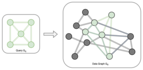
\includegraphics[width=\textwidth]{fig/LR/sgm-intro-double.png}
    \caption{Subgraph Enumeration Example}
    \label{fig:sgm-intro}
\end{figure}

Isomorphic graphs are of interest since they represent similarity between inherent topology of the graph.
% most graph properties do not depend on labels of vertices. \RN{<-unclear sentencee.}
% As graph data is mostly relational the similarity between inherent topology is captured by graph isomorphism. 
For graphs $G_1$ and $G_2$ graph isomorphism is a bijection between the vertex sets $\mathcal{V}(G_1)$ and $\mathcal{V}(G_2)$ $f: \mathcal{V}(G_1) \rightarrow \mathcal{V}(G_2) $ with the condition: \textit{any two vertices $u$ and $v$ of $G_1$ are adjacent in $G_1$ \textit{if and only if} $f(u)$ and $f(v)$ are adjacent in $G_2$}.
% Mathematically, for $G_1$ and $G_2$ to be isomorphic: $(u,v) \in \mathcal{E}(G_1) \leftrightarrow (f(u),f(v)) \in \mathcal{E}(G_2)$. Where \SV{Here,} $\mathcal{E}(.)$ represents the edge set of a graph. 
% \SV{Confusing. Maybe mention informally, define all the E, G terms first and then mathematically show what graph isomorphism is.} 
In this work we focus on undirected query graphs and data graphs.
Subgraph enumeration entails the subgraph isomorphism problem which is known to be NP-complete \cite{Book:Complexity_Theory}.

Subgraph Enumeration has wide range of applications.
For example, it can be used for plagiarism detection \cite{quasi-clique-plagiarism}, network motif counting \cite{motif-counting-application}, comparing similarity between large graphs \cite{large-graph-comparison-application}, designing bioinformatics networks \cite{bioinformatics-application}, chemical target structure synthesis \cite{chemical-target-application}, analyzing insights in recommendation networks \cite{recommendation-network-application}, etc.

% Demand for Data scalability
With the advent of \textit{Internet of Things} (IoT) and \textit{Information Technology} (IT), the sizes of graphs representing underlying data are substantially bigger and pose
%tough 
significant
challenges for data scalability.
Increasing interests in graph analytics and improvements to computational hardware over the last two decades, particularly in CPUs and GPUs have helped develop practical solutions to this computationally challenging problem.
Nevertheless, many existing solutions do not scale well with increasing template size due to issues like memory requirement, computational time, and load imbalance.

% My contribution

This work is focused on improving the existing state-of-the-art solution for subgraph enumeration: PARSEC, developed by Dodeja \etal \cite{PARSEC_VD}.
A series of enhancements were developed to improve its computational performance which are discussed in later sections. These enhancements include:
\begin{enumerate}
    \item Smart preprocessing techniques to detect intersection reuse and reduce computation.
          % \item Priority based sorting to reduce computation and eliminate overheads.
    \item Two-Phase strategy to improve symmetry breaking effectiveness.
    \item Hybrid parallelism for better load balance.
\end{enumerate}
%Rest of the chapters are 
The remainder of this thesis is organized as follows:
% Section summary
\begin{enumerate}[\indent {}]
    \item Chapter \ref{chap:Background} provides an overview of Graphics Processing Units and graph storage formats.
    \item Chapter \ref{chap:lit} is devotetd to a Literature Review that describes related work and defines mathematical notation used throughout this thesis.
    \item Chapter \ref{chap:basic-theory} illustrates basic techniques used in the subgraph enumeration algorithm with the help of a running example.
    \item Chapter \ref{chap:Improvements} describes the aforementioned enhancements in detail and analyzes their individual contribution to performance.
    \item Finally, Chapters \ref{chap:Results} and \ref{chap:conclusions} evaluate the combined improvement due to these individual enhancements and summarize the thesis with concluding remarks and scope for further work.
\end{enumerate}
